\documentclass[12pt,a4paper]{report}

% Pacotes básicos
\usepackage{mathptmx}
\usepackage[utf8]{inputenc}    % Permite acentuação
\usepackage[T1]{fontenc}       % Codificação correta das fontes
\usepackage[brazil]{babel}     % Idioma português
\usepackage{geometry}          % Configuração da página
\geometry{a4paper, top=2cm, bottom=2cm, left=2.5cm, right=2.5cm}
\usepackage{setspace}          % Espaçamento entre linhas
\usepackage{graphicx}          % Inserir imagens
\usepackage{hyperref}          % Links clicáveis
\usepackage{titlesec}          % Personalização dos títulos
\usepackage{array}             % Tabelas mais flexíveis
\usepackage{longtable}         % Tabelas longas
\usepackage{tikz}
\usetikzlibrary{positioning,shapes.geometric}

% Configurações do documento
\onehalfspacing               % Espaçamento 1.5
\hypersetup{
    colorlinks=true,
    linkcolor=blue,
    urlcolor=blue,
    pdftitle={Universidade Estadual do Norte Fluminense Darcy Ribeiro},
    pdfauthor={Davi Rodrigues Soares Machado},
}



% Título
\title{
	\begin{figure}
	\centering
	
\includegraphics[scale=0.3]{imagens/uenf1.png}
	\end{figure}
    \vspace{1cm}
    \Huge \textbf{Projeto da disciplina Paradigmas Orientados à Objetos para Desenvolvimento de Software} \\[0.5cm]
    \Large Sistema de Agenda Escolar
    \vspace{2cm}
}
\author{\textbf{Davi Rodrigues Soares Machado} \\ Ciência da Computação \\ LCMAT - CCT - UENF}
\date{\today}

\begin{document}

% Capa
\maketitle
\newpage

% Sumário
\tableofcontents
\newpage





%------------------------------------------------------------------------------------




% Introdução
\chapter{Introdução}
O objetivo por trás desse sistema é simular uma situação real de desenvolvimento para a disciplina Paradigmas Orientados à Objetos e Desenvolvimento de Software. A ideia do projeto é criar uma agenda escolar para uma rede de escolas, para que alunos, professores e outros profissionais possam visualizar e acompanhar informações como salas, turmas, professor responsável, entre outras funcionalidades que serão melhor demonstradas na sessão de \hyperref[sec:DCU]{Diagramas}. 


O desenvolvimento deste projeto será registrado dentro do github, onde será possível acompanhar a evolução do sistema através do \href{https://github.com/DaviRodrish/Projeto-PooDev---Agenda-Escolar}{Repositório Github}, seguindo o calendário disponível na sessão \hyperref[sec:Calendario]{Calendário}.


% Objetivos
\chapter{Objetivos}
O sistema tem como foco facilitar a gestão da agenda escolar, otimizando a alocação de salas, evitando conflitos de horários e permitindo que alunos e professores consultem suas grades. Conterá também recursos para os professores lançares as notas dos respectivos alunos. 
\section{Público Alvo}

\section{Orçamento}
% Levantamento de Requisitos
\chapter{Levantamento de Requisitos}
\section{Requisitos Funcionais}
\begin{itemize}
    \item RF01: Cadastrar professores, alunos, salas e disciplinas e unidades escolares.
    \item RF02: Consultar grade horária por aluno, professor ou sala.
    \item RF03: Alocar salas a disciplinas em horários específicos.
    \item RF04: Impedir conflitos de agendamento.
    \item RF05: Gerir notas dos alunos, sendo possivel gerar relatorios com situaçao de aprovado ou reprovaado ou registro de notas.
    \item RF05: Sistema de assinatura digital dos professores e coordenadores.
\end{itemize}

\section{Requisitos Não Funcionais}
\begin{itemize}
    \item RNF01: O sistema deve ser responsivo e rápido.
    \item RNF02: Deve funcionar em navegadores modernos.
    \item RNF03: Os dados devem ser armazenados de forma segura.
\end{itemize}

% Casos de Uso
\chapter{Diagramas}
\section{Diagrama de Caso de Uso}
\label{sec:DCU}
No diagrama abaixo estão os principais tipos de usuários, com os respectivos elementos que cada um terá acesso dentro do sistema
\begin{figure}[h!]
\centering
\includegraphics[width=.9\textwidth]{imagens/aluno.png}
\caption{Diagrama de Casos de Uso}
\label{Diagrama de Casos de Uso}
\end{figure}



% Arquitetura do Sistema
\chapter{Arquitetura do Sistema}
O aplicativo será desenvolvido utilizando \textbf{React} no front-end e \textbf{Node.js} no back-end, com banco de dados \textbf{PostgreSQL}.  
A comunicação entre os módulos será feita por meio de \textbf{API REST}.

% Tecnologias Utilizadas
\chapter{Tecnologias Utilizadas}
\begin{itemize}
    \item \textbf{Front-end:} React + Tailwind CSS
    \item \textbf{Back-end:} Node.js + Express
    \item \textbf{Banco de Dados:} PostgreSQL
    \item \textbf{Controle de Versão:} GitHub
\end{itemize}

% Calendário
\chapter{Calendário}
\label{sec:Calendario}

Para melhor entendimento, o calendário de desenvolvimento foi dividido em dois bimestres, sendo o primeiro focado em backend e integração com banco de dados, e o segundo focado no frontend e nos testes de aplicação. Em ambas etapas, no final de cada semana do mês, uma reunião com cliente irá acontecer, onde será mostrado cada nova parte incluída no sistema.  

\vspace{2cm}

\begin{figure}[h!]
\centering
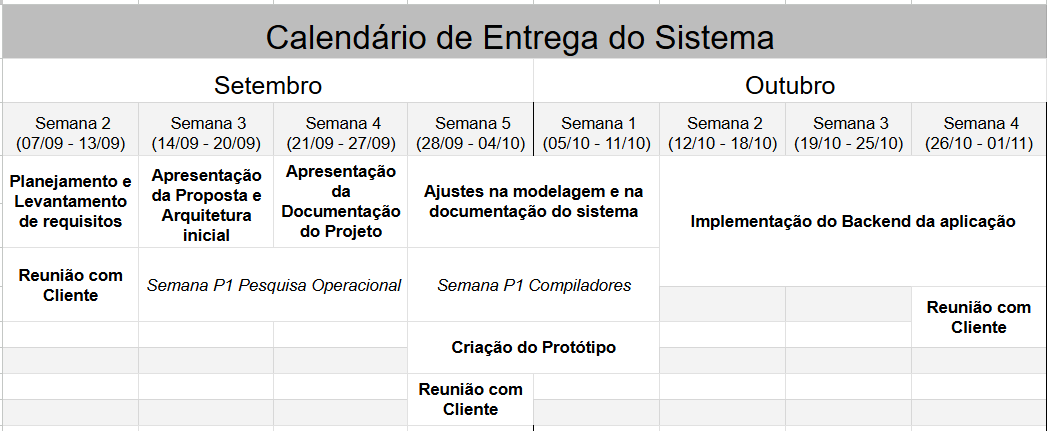
\includegraphics[width = \linewidth]{imagens/Calendario1bi.png}
\caption{Calendário Primeiro Bimestre de Desenvolvimento}
\label{Calendário Primeiro Bimestre de Desenvolvimento}
\end{figure}

\begin{figure}[h!]
\centering
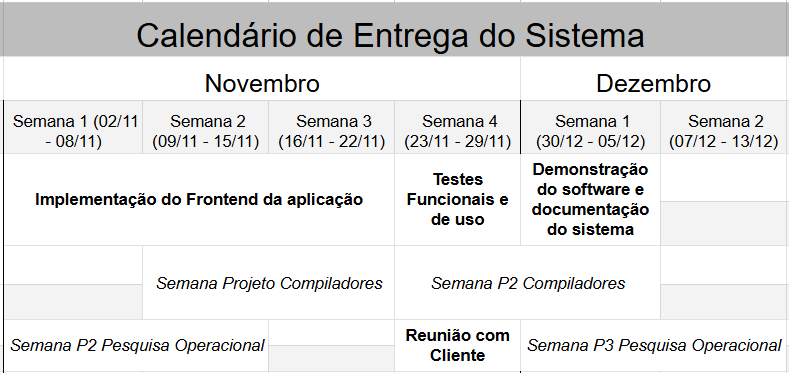
\includegraphics[width = \linewidth]{imagens/Calendario2bi.png}
\caption{Calendário Segundo Bimestre de Desenvolvimento}
\label{Calendário Segundo Bimestre de Desenvolvimento}
\end{figure}

% Conclusão
\chapter{Conclusão}
Esta documentação serve como referência para o desenvolvimento e manutenção do aplicativo, garantindo clareza nos requisitos e funcionalidades.

\end{document}
